\chapter*{Deuxième Partie : Le corpus et données : l’exemple de l’année 2022}
\setcounter{chapter}{2}  % Đặt lại số chương thành 2
% images, schema, Lucidchart pour faire des schémas

\section{Présentation du corpus : Journaux Officiels 2022}

Au cœur de cette étude se trouve les Journaux Officiels (JO) de l'année 2022, qui sont comptes rendu intégraux des séances plénière en 2022. Ce corpus constitué de 86 fichiers totalisant 8485 pages.

Le texte brut des comptes rendus est disponible au format WORD, mais après publication, les fichiers sont accessibles à la fois en \gls{PDF} et en une seule page \gls{HTML} depuis le site officiel du Sénat : \url{https://www.senat.fr/seances/seances.html}.
De plus, une version \gls{XML} de ces documents est transmise pour l'intégration dans la base de données officielle du Sénat, et est accessible directement depuis leur site web : \url{https://data.senat.fr/la-base-comptes-rendus/}.
Au-delà de leur diversité de formats et de mise en page, ces documents partagent tous un même contenu. Après avoir lu différents formats pour identifier les détails à extraire, ainsi que la structure propre à chaque format, il a été conclu que la version du document au format \gls{PDF} serait principalement utilisée dans le processus d'extraction automatique. En effet, ce choix repose sur l'exhaustivité des détails et leur intégration dans un texte facile à analyser de manière automatique. Concernant le format WORD, la forme et la structure ne sont pas adaptées au traitement automatique, car le contenu n'est pas divisé en colonnes, la taille et la police des caractères ne sont pas toujours correctement configurées, enfin, les numéros de page ne sont pas marqués.
Par ailleurs, les fichiers \gls{HTML} et \gls{XML} ne sont pas structurés en colonnes et ne comportent pas de numéros de page. Cependant, la lecture et l'enregistrement des balises de données au format \gls{XML} peuvent faciliter l'intégration des informations extraites dans des bases de données ou des systèmes de pré-publication après extraction.

\subsection{Pourquoi avoir choisi d’expérimenter sur les documents de 2022}

Le choix de l'année 2022, année faisant suite à deux ans marqués par la pandémie de Covid-19, s'explique par le fait que les sujets discutés reprennent alors un cours plus normal, se détachant des questions sanitaires pour mieux se recentrer sur des enjeux de long terme au cœur des débats.

De plus, après avoir échangé avec le directeur des archives, Jean-Marc Tichi, et l'équipe des archives, le choix de l'année 2022 s'explique également par le fait qu'il s'agit d'une année récente pour laquelle Mme Ghislaine Laumonerie a encore conservé quelques Journaux Officiels au format papier, car ceux des années antérieures n'ont plus tous été gardé physiquement. Cela nous permet donc de montrer clairement les annotations manuscrites sur les Journaux Officiels et de mieux comprendre les détails du processus de travail en équipe. Elle précise que l'année 2023 ne pouvait pas être utilisée, car elle n'était pas encore entièrement traitée au début du stage en avril 2024. Il était important d'éviter toute interférence avec le travail en cours sur les Journaux Officiels de 2023 et l'élaboration de la Table nominative de 2023.


\section{Étude des Corpus}

Nous avons effectué une lecture rapide du document afin de localiser des éléments clés comme la table des matières, les titres des sections et sous-sections, afin de mieux comprendre la structure générale du document ainsi que ses sections principales, et mieux saisir l'organisation du contenu pour accéder rapidement aux informations essentielles. Après avoir lu plusieurs exemples, nous avons une vision claire du format commun et de la structure de tous les JOs. Cette approche nous a permis d'identifier des informations cruciales, notamment le nom des intervenants, les dates, les textes de loi, les sujets de discussions, etc...

\subsection{Structure générale d'un compte rendu}
La structure générale d'un fichier de compte rendu comprend plusieurs éléments. La page de titre contient : le titre, la date de la séance, la date de publication du \gls{JO} ainsi qu'une image du Sénat sur la couverture. Le contenu principal est organisé avec, sur chaque page, un en-tête comprenant le titre, la date et la session. Les parties principales incluent un sommaire qui liste les sujets abordés et les intervenants, un compte rendu intégral des débats, et des annexes (facultatif).

Les documents parlementaires ou les rapports officiels sont divisés en plusieurs colonnes pour organiser le texte. Dans le cas de ce document, le contenu est souvent disposé en deux colonnes principales. Cela permet de gagner de la place au moment de l'impression. Le document est structuré en fonction des séances ou des jours de réunion, avec des titres clairs comme "Séance du [date]" pour indiquer la date de la séance. Cela permet de retrouver clairement les informations relatives à une séance spécifique. Cependant, la mise en signet se poursuivra de session en session. Les numéros de page sont marqués de la première séance à la dernière séance de l'année et le marquage des pages sera repris à la première séance de l'année suivante.

\subsection{Éléments de contenu principaux dans le texte}

\begin{figure}[H]
    \centering
    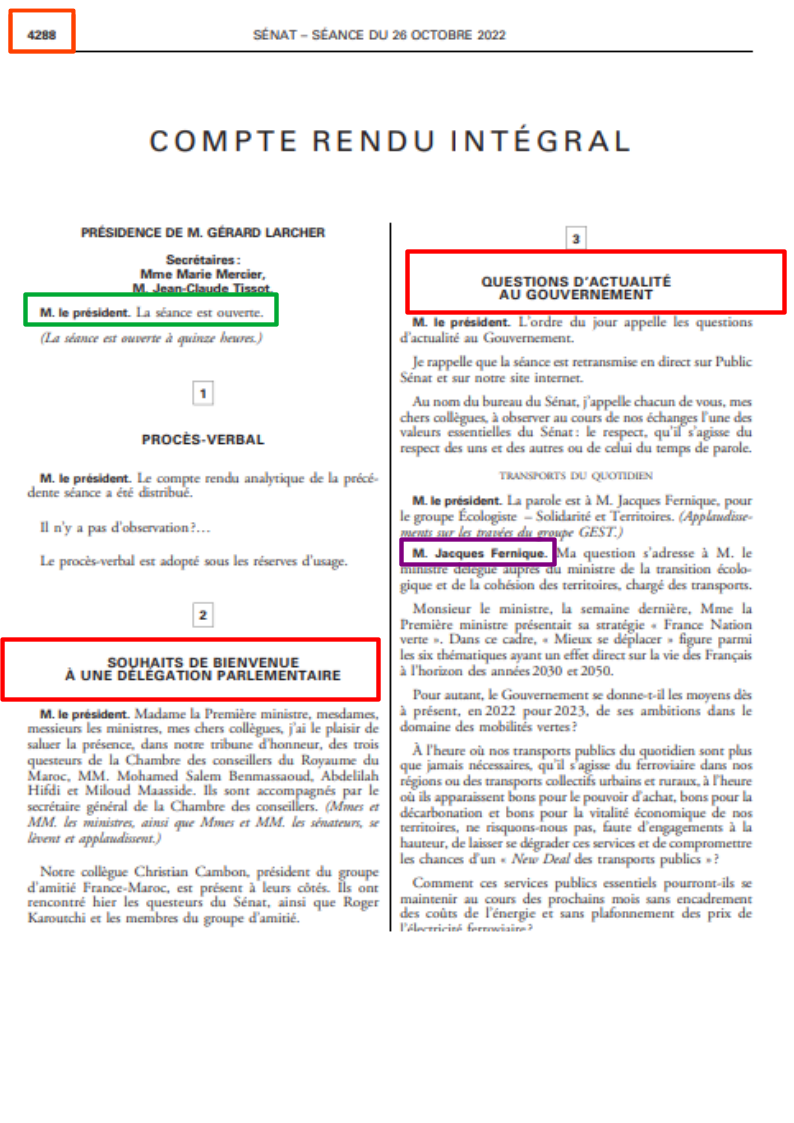
\includegraphics[width=0.7\textwidth]
    {images/structure.png}
    \caption{Capture de JO du 26 octobre 2022}
\end{figure}

\paragraph{Noms des intervenants} Les noms apparaissent souvent sous la forme "M. [Nom]" ou "Mme [Nom]" et sont en gras ou clairement distingués pour être facilement identifiables. Après le nom suit la prise de parole ou l’échange de cet intervenant.

\paragraph{Sujets de discussion} Dans chaque séance, les sujets principaux sont clairement présentés à travers des titres écrits en majuscules et centrés sur la page en dessous du numéro du titre encadré . Par exemple, des sections comme "SOUHAITS DE BIENVENUE À UNE DÉLÉGATION PARLEMENTAIRE" ou "QUESTIONS D’ACTUALITÉ AU GOUVERNEMENT" sont toujours bien visibles, permettant aux lecteurs d'identifier rapidement les différentes parties du débat. Cette présentation structurée aide à naviguer efficacement dans les discussions et à suivre le déroulement des séances parlementaires.

\paragraph{Numéro de pages} Le numéro de pages est systématiquement placé en tête de chaque page dans les documents officiels, facilitant ainsi la navigation et la référence. La numérotation est continue à partir de la première séance de l'année jusqu'à la dernière, sans interruption, ce qui permet de suivre les débats et les décisions de manière cohérente tout au long de l'année législative. Ce système assure une traçabilité et une transparence dans l'organisation des séances.

\paragraph{Subdivision du texte} Les sections sont divisées en petits paragraphes, souvent marqués par des titres ou des numéros d’articles ou d’amendements (par exemple, "Article 1er").

\paragraph{Nature de texte} La nature de textes de loi qui écrit en majuscule et dessus de textes de lois

\begin{figure}[H]
    \centering
    \includegraphics[width=0.45\textwidth]{images/Article.png}
    \caption{Capture de JO du 26 octobre 2022}
\end{figure}

\section{Défis pour l’automatisation}

\subsection{Les tâches à automatiser}
% Ajouter une sous partie sur le recueil des besoins : ici, décrire dans le détails ce dont a besoin le service d'archives et synthèse détaillée de ses besoins.

Dans ce projet, les tâches ont été divisées en deux parties principales : \textbf{la première partie} concerne l'extraction des informations telles que le nom des intervenants et les numéros de page à partir des Journaux Officiels (JOs), et \textbf{la deuxième partie} se concentre sur l'entraînement des modèles de machine learning pour générer des thèmes à partir des textes parlementaires.

\subsubsection{Première Partie : Extraction d'Informations des Journaux Officiels}

\paragraph{Rassembler les Journaux Officiels 2022}  
Avant de commencer l'extraction des informations, il est essentiel de rassembler et de télécharger tous les Journaux Officiels (JOs) complets de l'année 2022 au format \gls{PDF} à partir du site officiel du Sénat. Pour télécharger des fichiers en masse depuis un site web, nous pouvons utiliser la technique du grattage de données web, \textit{web scraping} pour extraire automatiquement les données ou télécharger les fichiers de ce site. Cette étape de collecte garantit que nous avons à disposition l'ensemble des documents nécessaires pour les étapes d'extraction et d'analyse ultérieures. 

\paragraph{Extraction du texte des fichiers \gls{PDF}}  
Pour commencer l'analyse, l'extraction du texte des fichiers \gls{PDF} est une tâche cruciale, car ces fichiers contiennent des informations lisibles nécessaires à l'analyse. Nous avons décidé de tester plusieurs bibliothèques pour le traitements les documents pdf pour cette tâche. Il faut trouver une \gls{bibliothèque} qui a sa capacité à extraire du texte de manière fiable à partir de fichiers \gls{PDF} complexes tout en maintenant la structure du document. Le temps estimé pour cette tâche est de deux semaines, avec une semaine supplémentaire pour les ajustements.

\paragraph{Nettoyage du texte}  
Une fois le texte extrait, il est nécessaire de le nettoyer. Cette tâche consiste à supprimer les sections du texte qui ne sont pas pertinentes pour l'analyse, spécifiquement les lignes qui commencent par "M. le président. La séance est ouverte" et celles qui se terminent par "La séance est levée". Cette étape est essentielle pour s'assurer que seuls les contenus pertinents sont conservés pour l'analyse ultérieure. Nous pouvons donc supprimer ces lignes grâce à un script qui fera le filtrage du texte automatiquement à partir de ces mots-clés.

\paragraph{Numérotation des noms des intervenants}  
La numérotation des noms des intervenants est une tâche technique complexe. Initialement, nous avons utilisé le modèle NLP de \gls{spaCy} pour identifier et numéroter les noms des intervenants à travers la reconnaissance des entités nommées (NER). Cependant, les tests avec \gls{spaCy}, \gls{BERT}, et \gls{gliner} ont montré des limites, notamment la perte de nombreux noms et la présence de nombreuses erreurs. Face à ces défis, nous avons décidé de retourner aux fichiers \gls{PDF} d'origine et d'utiliser la bibliothèque \gls{pdfplumber} combinée avec des expressions régulières (\gls{regex}) pour compter et numéroter les noms des intervenants dans les Journaux Officiels (JOs). Le processus de numérotation des intervenants est prévu pour se terminer entre le 5 et le 8 juillet 2024.

\paragraph{Extraction des noms des intervenants}  
L'extraction des noms des intervenants à partir des fichiers \gls{PDF} a été réalisée en utilisant \gls{pdfplumber}. Cette tâche, bien qu'étant relativement similaire à la numérotation des noms, a nécessité une approche légèrement différente pour garantir la précision des résultats. L'extraction devrait être finalisée d'ici le 8 juillet 2024.

\paragraph{Extraction des dates de séances}  
Pour extraire les dates des séances, nous avons opté pour une approche basée sur les noms de fichiers, chaque fichier étant nommé selon le format "sYYYYMMDD". Cette méthode simple mais efficace permet de récupérer rapidement les dates des séances pertinentes.

\paragraph{Enregistrement des numéros de page pour chaque intervention}  
Cette tâche implique plusieurs étapes complexes. Tout d'abord, le programme extrait les lignes de texte en gras de chaque page du fichier \gls{PDF}, en utilisant \gls{pdfplumber} pour identifier les caractères appartenant à une police en gras. Ensuite, ces lignes sont analysées pour extraire les honorifiques tels que "Mme le", "M.", "Mme", ainsi que les numéros de page correspondants. Ce processus est essentiel pour cartographier correctement les interventions dans les comptes rendus.

\paragraph{Enregistrement des documents par noms de sénateur/sénatrice}  
Une fois toutes les données extraites et nettoyées, elles seront enregistrées dans des fichiers \gls{CSV}, classés par noms de sénateurs et sénatrices. Cette étape finale permettra d'organiser les informations de manière cohérente pour une analyse plus approfondie.

\subsubsection{Deuxième Partie : Entraînement des Modèles de Machine Learning pour la Création de Thèmes}

\paragraph{Collecte des articles additionnels et des rapports}  
Cette tâche consiste à rechercher et télécharger manuellement chaque texte pertinent depuis le site officiel du Sénat. Les documents à récupérer incluent les articles additionnels et les rapports complémentaires liés aux débats parlementaires.

\paragraph{Identification / extraction des thèmes de projets de loi et des rapports supplémentaires} .\\
Pour identifier et extraire les thèmes des projets de loi et des rapports supplémentaires, nous envisageons d'utiliser des modèles de traitement du langage naturel (NLP) comme \gls{BERT}, \gls{spaCy}, ou même \gls{ChatGPT}. Ces outils permettront de classifier et d'extraire les thèmes principaux des textes analysés.

\paragraph{Sauvegarde des résultats en fichiers \gls{CSV}}.\\
Après l'extraction des thèmes, les résultats seront sauvegardés sous forme de fichiers \gls{CSV}. Pour accomplir cette tâche, nous utiliserons la \gls{bibliothèque} \texttt{csv} de Python, qui permet une manipulation simple et efficace des données sous ce format. Le choix du format \gls{CSV} est crucial pour assurer une compatibilité élevée et faciliter l'accès aux données pour les utilisateurs finaux, tout en conservant une structure standardisée et facilement manipulable des données par divers logiciels et outils d'analyse. 

\subsection{Tâches Sélectionnées et Justifications}

Dans ce projet, nous avons choisi de nous concentrer sur les tâches décrites dans la première partie, à savoir l'extraction d'informations telles que les noms des intervenants, les numéros de page, les dates des séances ainsi que la numérotation des intervenants dans chaque session à partir des \textit{Journaux Officiels} (JOs). La raison principale de ce choix est que ces informations sont déjà présentes dans un format structuré au sein des JOs, ce qui permet de les traiter, d'analyser et d'extraire de manière plus précise et efficace sans avoir besoin de consulter d'autres sources externes ou d'examiner des documents supplémentaires.

Ces tâches sont particulièrement adaptées pour un projet de stage car elles se concentrent sur un domaine spécifique avec des données bien définies. Elles offrent ainsi une excellente opportunité de développer des compétences en matière de traitement et d'extraction d'informations, notamment la numérotation des intervenants dans chaque séance, tout en étant suffisamment accessibles pour être réalisées dans le cadre d'un mémoire de fin d'études. De plus, ce type de tâches garantit un haut niveau de précision dans l'extraction des données, ce qui est crucial pour produire un travail de qualité et validé sur le plan académique.

Enfin, le choix de ces tâches permet de travailler dans un périmètre maîtrisable, tant au niveau du volume des données à traiter que de la complexité des outils à utiliser. Cela correspond parfaitement aux attentes et aux contraintes d'un stage de fin d'études, tout en facilitant la rédaction d'un mémoire qui pourra être présenté pour valider l'année universitaire.


\subsection{Tâches Non Réalisables et Raisons}

La deuxième partie du projet ne pourra pas être réalisée pour l'ensemble du corpus et incluse dans le mémoire. La raison principale est que l'encodage et la recherche des projets de loi de 2022 ne sont pas centralisés dans une seule liste, ni sur une page unique, ce qui rend leur récupération extrêmement chrono-phage. De plus, ces projets de loi sont dispersés à la fois à l'extérieur et à l'intérieur des Journaux Officiels (JOs), ce qui complique davantage l'analyse et la distinction entre les différents types de titres. La fragmentation des informations entre plusieurs sources impose un travail manuel de consolidation, un processus long et complexe à effectuer avec des ressources limitées. Cette tâche dépasse largement les possibilités d'un projet de stage réalisé dans un délai restreint.

Par ailleurs, le temps et les compétences techniques actuellement disponibles sont encore insuffisants. Mener à bien cette tâche exigerait non seulement une durée considérablement plus longue, mais aussi l'intervention d'un spécialiste en technologies de l'information, capable de développer des outils spécifiques pour automatiser certaines étapes, telles que la récupération des projets de loi dispersés ou la différenciation des titres complexes. De plus, avec un corpus de cette taille et l'utilisation d'outils pour la génération de thèmes, il serait nécessaire de mettre en place des modèles d'apprentissage automatique avancés. Ces modèles requièrent des ressources informatiques bien supérieures à celles d'un simple ordinateur portable. En effet, l'entraînement de modèles complexes demande une puissance de calcul importante, généralement disponible uniquement sur des serveurs spécialisés ou des infrastructures de dans le \gls{cloud}. Cela dépasse donc les capacités matérielles à disposition dans le cadre de ce stage.


